\section{Auswertung}
\label{sec:auswertung}
In diesem Versuch werden zwei Temperatur-Strom-Kurven mit unterschiedlichen Heizraten $b$ analysiert.
Messreihe A hat eine Heizrate von $b_{\text{A}}=\SI{2}{\kelvin\per\minute}$ und es wird in dem Temperaturbereich
$T\in\left[\SI{213.1}{\kelvin},\SI{330.3}{\kelvin}\right]$ gemessen. Für Messreihe B beträgt die Heizrate
$b_{\text{B}}=\SI{1}{\kelvin\per\minute}$ und der vermessene Temperaturbereich ist $T\in\left[\SI{232.7}{\kelvin},\SI{289.6}{\kelvin}\right]$.
In beiden Fällen ist Kaliumbromid $\ce{KBr}$ der verwendete Kristall. Die Messdaten sind in Tabelle \ref{tab:Messdaten_roh}
abgebildet. 
\subsection{Bestimmung des Untergrundes}
Um den Untergrund zu bestimmen wird die Exponentialfunktion
\begin{equation}
    I_{\text{U}}(T) = C\cdot\exp\left(D\cdot  T\right)
\end{equation}
an die Messdaten vor und nach dem Peak gefittet.
Die Messdaten und die Fits sind in Abbildung \ref{fig:Untergrund_A} und \ref{fig:Untergrund_B} dargestellt.
\FloatBarrier
\begin{figure}
    \centering
    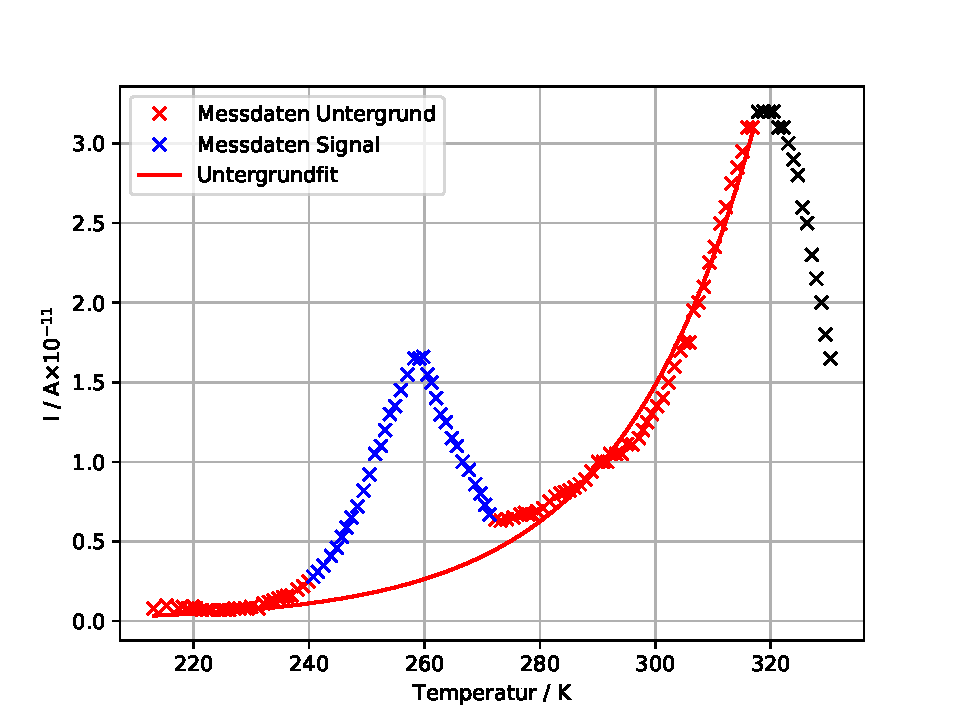
\includegraphics[width =0.8\textwidth, keepaspectratio]{figure/Untergrund_A.pdf}
    \caption{Messdaten und Untergrundfit für Messreihe A. Hierbei können die Messdaten nach dem zweiten Peak nicht für die 
    Bestimmung des Untergrundes verwendet werden.}
    \label{fig:Untergrund_A}
\end{figure}
\begin{figure}
    \centering
    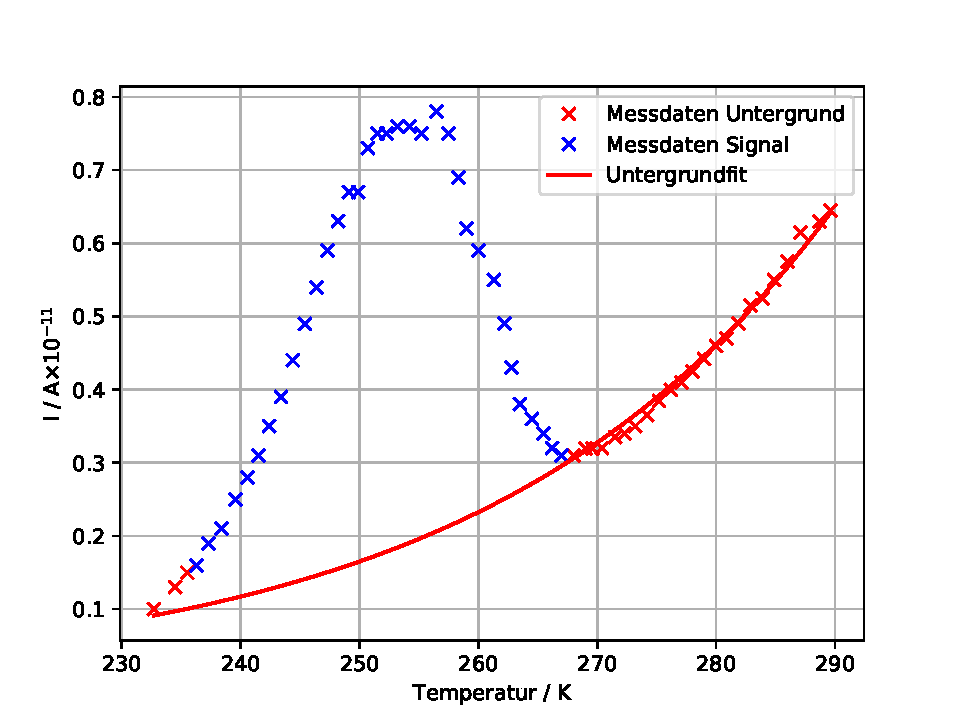
\includegraphics[width =0.8\textwidth, keepaspectratio]{figure/Untergrundfit_B.pdf}
    \caption{Messdaten und Untergrundfit für Messreihe B.}
    \label{fig:Untergrund_B}
\end{figure}
\FloatBarrier
Die Fitparameter sind in der Tabelle \ref{tab:Fit_params_untergrund} aufgelistet.
\begin{table}
    \centering
    \caption{Fitparameter für die Untergrundfunktionen der beiden Messreihen.}
    \label{tab:Fit_params_untergrund}
    \begin{tabular}{c c c}
        \toprule
        Messreihe &$C\,/\,\SI{}{\ampere}$&$D\,/\,\SI{}{\per\kelvin}$\\
        \midrule
        A&$\num{3.5(9)e-6}$&$\num{0.0431(8)}$\\
        B&$\num{3.1(9)e-5}$&$\num{0.0343(10)}$\\
        \bottomrule
    \end{tabular}
\end{table}
\FloatBarrier
Um die Messreihe vom Untergrund zu bereinigen, werden von den gemessenen Stromwerten die Werte der Untergrundfunktion subtrahiert.
Die bereinigten Messwerte sind in Abbildung \ref{fig:Messdaten_bereinigt_A}
und \ref{fig:Messdaten_bereinigt_B} zu sehen.
\FloatBarrier
\begin{figure}
    \centering
    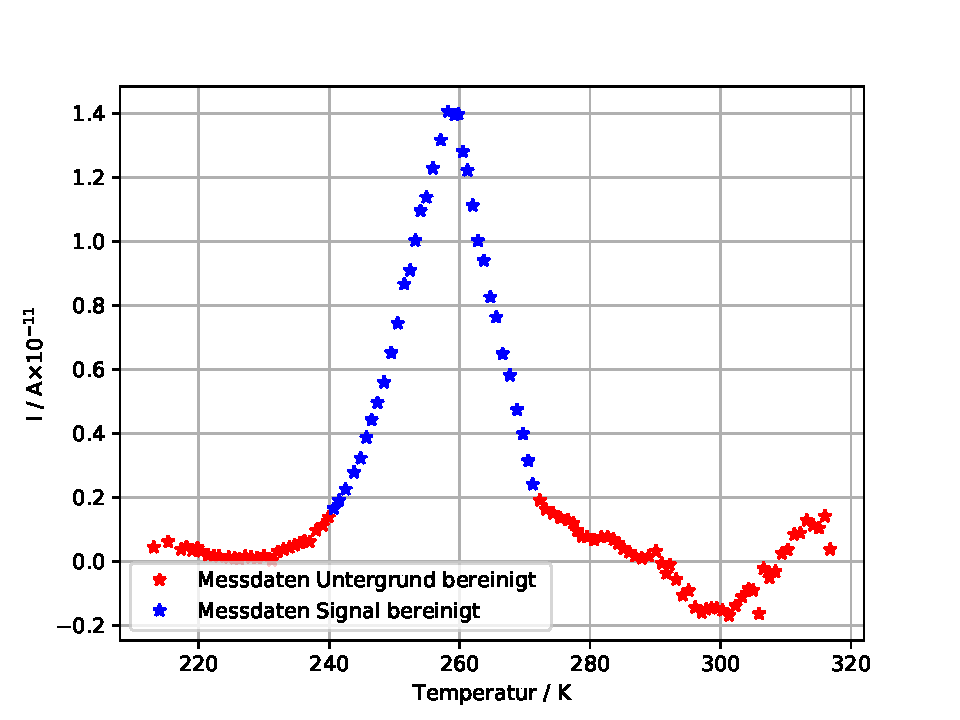
\includegraphics[width=0.8\textwidth,keepaspectratio]{figure/Messdate_rein_A.pdf}
    \caption{Vom Untergrund bereinigte Messdaten der Messreihe A.}
    \label{fig:Messdaten_bereinigt_A}
\end{figure}
\begin{figure}
    \centering
    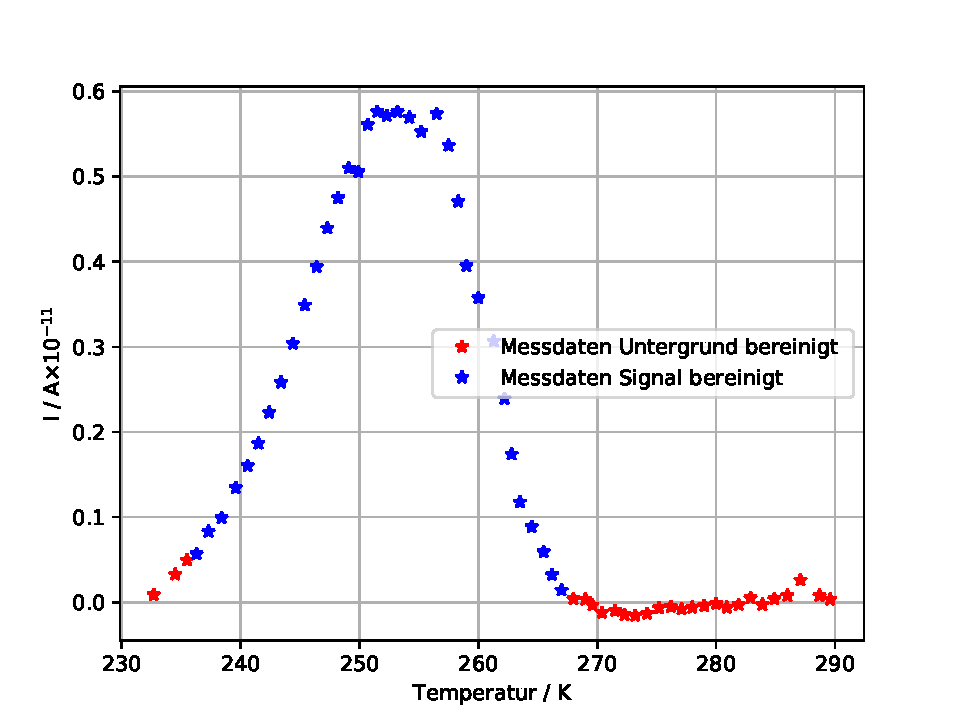
\includegraphics[width=0.8\textwidth,keepaspectratio]{figure/Messdate_rein_B.pdf}
    \caption{Vom Untergrund bereinigte Messdaten der Messreihe B.}
    \label{fig:Messdaten_bereinigt_B}
\end{figure}
\FloatBarrier

\subsection{Niedertemperaturapproximation}
Um die Aktivierungsenergie $W$ zu ermittelt, wird Gleichung \eqref{eq2} verwendet.
Dafür werden die bereinigten Messdaten der Messreihe A im Bereich $T_{\text{A}}\in \left[\SI{232.2}{\kelvin},\SI{253.2}{\kelvin}\right]$
und für Messreihe B im Bereich von $T_{\text{B}}\in \left[\SI{232.7}{\kelvin},\SI{250.7}{\kelvin}\right]$ logarithmiert und gegen $\frac{1}{T}$ aufgetragen.
Dazu wird eine lineare Ausgleichsgerade 
\begin{equation*}
    \text{ln}\left(I(T)\right) = \frac{-W}{k_{\text{{B}}}} \frac{1}{T} +\beta
\end{equation*}
angepasst. Hierbei ist der Fitparameter $W$ die Aktivierungsenergie des Kristalls.
Die logarithmiert Messdaten und die Ausgleichsgrade sind in den Abbildungen \ref{fig:Lin_fit_W_A} und \ref{fig:Lin_fit_W_B}
abgebildet.
\FloatBarrier
\begin{figure}
    \centering
    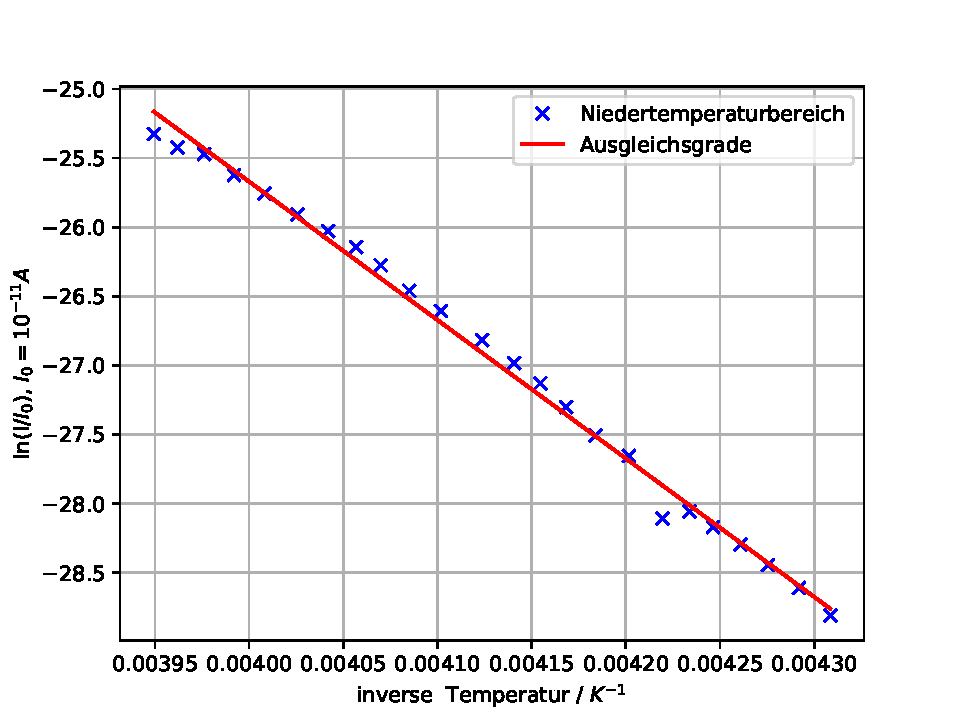
\includegraphics[width=0.8\textwidth,keepaspectratio]{figure/LinFit_W_A.pdf}
    \caption{Messdaten und lineare Ausgleichsgrade für die Bestimmung der Aktivierungsenergie $W$ mit Hilfe der Messreihe A.}
    \label{fig:Lin_fit_W_A}
\end{figure}
\begin{figure}
    \centering
    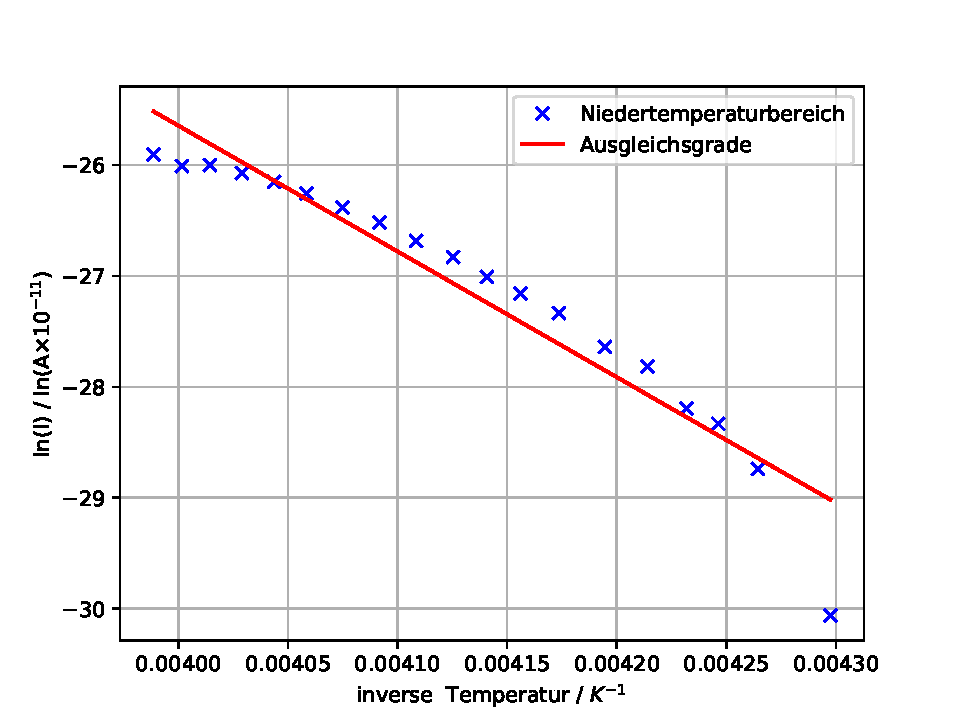
\includegraphics[width=0.8\textwidth,keepaspectratio]{figure/LinFit_W_B.pdf}
    \caption{Messdaten und lineare Ausgleichsgerade für die Bestimmung der Aktivierungsenergie $W$ mit Hilfe der Messreihe B.}
    \label{fig:Lin_fit_W_B}
\end{figure}
\FloatBarrier
Die Fitparameter sind in Tabelle \ref{tab:Niedertemperatur_approx_fit_params} abgebildet.
\begin{table}
    \centering
    \caption{Fitparameter der linearen Ausgleichsgeraden der beiden Messreihen.}
    \label{tab:Niedertemperatur_approx_fit_params}
    \begin{tabular}{c c c c}
        \toprule
        Messreihe & $\beta \,/\, \ln(\SI{e-11}{\ampere})$&$W \,/\,\SI{}{\joule}$&$W \,/\,\SI{}{\milli\eV}$\\
        \midrule
        A&$\num{14.4(7)}$&$\num{1.383(23)e-19}$&$\num{863(14)}$\\
        B&$\num{19.7(34)}$&$\num{1.57(11)e-19}$&$\num{980(70)}$\\
        \bottomrule
    \end{tabular}
\end{table}
\newpage
\subsection{Integrationsverfahren}
Bei dieser Methode wird die Aktivierungsenergie mithilfe von Gleichung \eqref{eq3}  bestimmt.
Das Integral aus Gleichung \eqref{eq3} wird numerisch mittels der Trapezregel bestimmt.
An die ermittelten Daten wird eine lineare Ausgleichsgerade der Form 
\begin{equation*}
    \ln{ \left( \frac{ \int_{T}^\infty j(T') \mathrm{d}T' }{ b j(T) \tau_{\text{0}} } \right) } = \frac{W}{k_{\text{{B}}}} \frac{1}{T} +\beta
\end{equation*}
angepasst. Der Fitparameter $W$ ist die Aktivierungsenergie.
Die Messdaten und die Fits sind in den Abbildungen \ref{fig:Integralverfahren_A} und \ref{fig:Integralverfahren_B} abgebildet.
\FloatBarrier
\begin{figure}
    \centering
    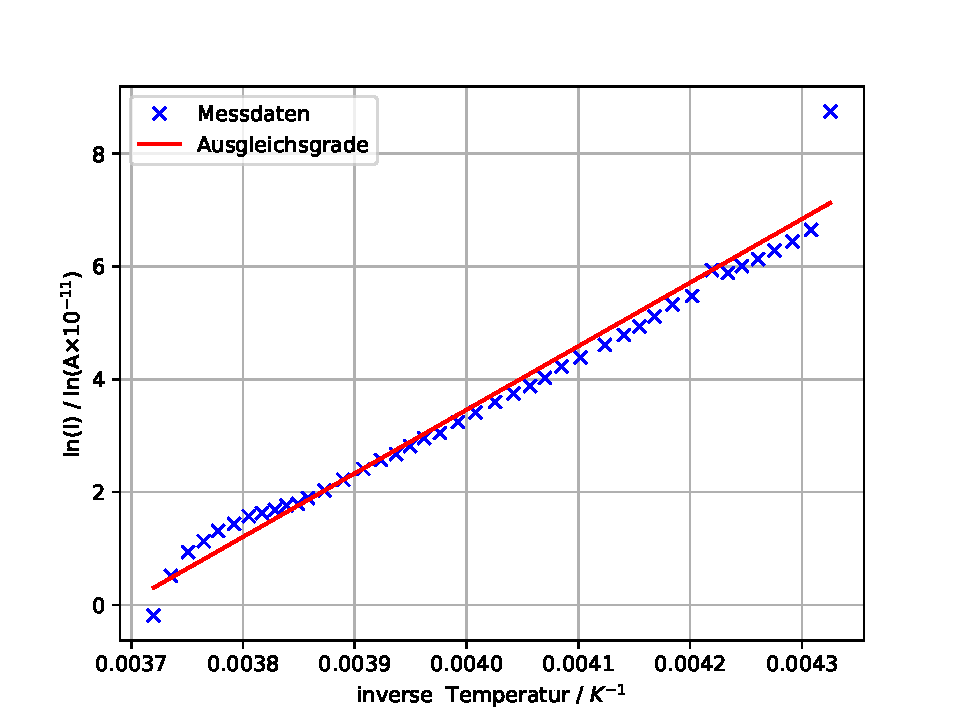
\includegraphics[width= 0.8\textwidth,keepaspectratio]{figure/Integralverfahren_A.pdf}
    \caption{Messdaten und lineare Ausgleichsgerade für die Bestimmung der Aktivierungsenergie mithilfe des Integrationsverfahrens für Messreihe A.}
    \label{fig:Integralverfahren_A}
\end{figure}
\begin{figure}
    \centering
    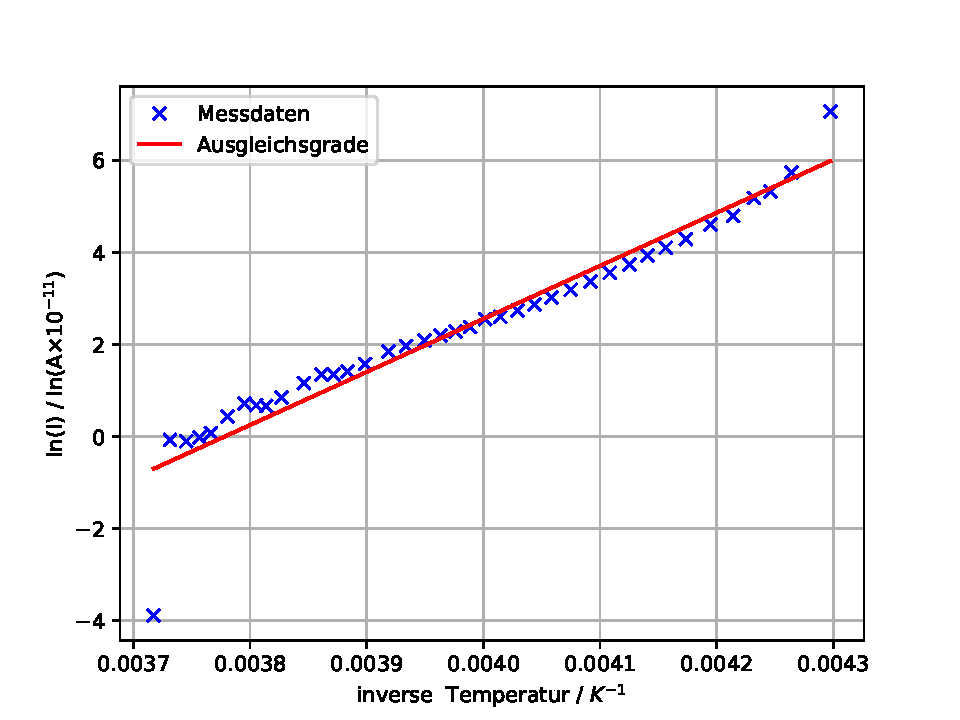
\includegraphics[width= 0.8\textwidth,keepaspectratio]{figure/Integralverfahren_B.pdf}
    \caption{Messdaten und lineare Ausgleichsgerade für die Bestimmung der Aktivierungsenergie mithilfe des Integrationsverfahrens für Messreihe B.}
    \label{fig:Integralverfahren_B}
\end{figure}
\FloatBarrier
Die Fitparameter der Ausgleichsgeraden aus denn Abbildungen \ref{fig:Integralverfahren_A} und \ref{fig:Integralverfahren_B} sind 
in Tabelle \ref{tab:Fit_params_integtal} aufgelistet.
\begin{table}
    \centering
    \caption{Fitparameter der Ausgleichsgeraden für die Bestimmung der Aktivierungsenergie mithilfe des Integrationsverfahrens.}
    \label{tab:Fit_params_integtal}
    \begin{tabular}{c c c c}
        \toprule
        Messreihe&$\beta \,/\, \ln(\SI{e-11}{\ampere})$&$W \,/\,\SI{}{\joule}$&$W \,/\,\SI{}{\milli\eV}$\\
        \midrule
        A&$\num{-41.6(14)}$&$\num{1.56(5)e-19}$&$\num{971(30)}$\\
        B&$\num{-43.6(23)}$&$\num{1.59(8)e-19}$&$\num{990(50)}$\\
        \bottomrule
    \end{tabular}
\end{table}
\newpage
\subsection{Bestimmung der Relaxationszeit \texorpdfstring{$\tau_{0}$}{T1}}
Um die Relaxationszeit $\tau_{0}$ zu bestimmen wird die Funktion \eqref{eq:j_T} nach der Temperatur abgeleitet und 
die Temperatur beim Strommaximum eingesetzt und gleich Null gesetzt.
\begin{gather*}
    \left.\frac{\text{d}j(T)}{\text{d}T}\right|_{T_{\text{max}}}=0\\
    \implies \tau_0 = \frac{k_{\text{B}}T_{\text{max}}^2}{Wb}\exp{\left(-\frac{W}{k_{\text{B}}T_{\text{max}}}\right)}
\end{gather*}
$\tau_0$ wird mit den vorher bestimmten Ergebnissen der verschiedenen Methoden bestimmt.
Die verschiedenen $\tau_0$-Werte sind in Tabelle \ref{tab:tau_0} aufgelistet.
\FloatBarrier
\begin{table}
    \centering
    \caption{$\tau_0$-Werte der beiden Messreihen für die zwei Methoden zur Bestimmung der Aktivierungsenergie.}
    \label{tab:tau_0}
    \begin{tabular}{c c c}
        \toprule
        Messreihe&$\tau_0\,/\,\SI{}{\second}$ (Approximationsverfahren)&$\tau_0\,/\,\SI{}{\second}$ (Integrationsverfahren)\\
        \midrule
        A&$\num{2.8(18)e-15}$&$\num{2.0(27)e-17}$\\
        B&$\num{8(30)e-18}$&$\num{4(9)e-18}$\\
        \bottomrule
    \end{tabular}
\end{table}
\FloatBarrier
Die Unsicherheiten sind sehr groß im Vergleich zu den bestimmten Werten, darauf wird in der Diskussion eingegangen.
Mit den $\tau_0$- und den $W$-Werten kann der Verlauf $\tau(T)$ dargestellt werden.
Diese sind in Abbildung \ref{fig:tau_verlauf_A} und \ref{fig:tau_verlauf_B} zu sehen.
\FloatBarrier
\begin{figure}
    \centering
    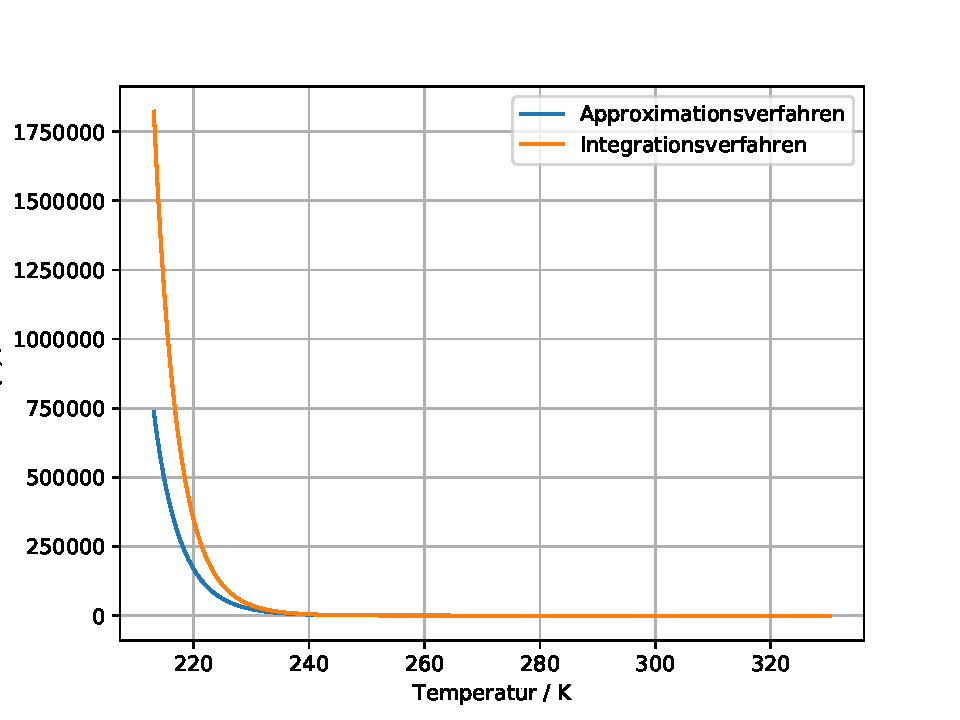
\includegraphics[width = 0.8\textwidth , keepaspectratio]{figure/tau_verlauf_A.pdf}
    \caption{Verlauf der Relaxationszeit für die Messreihe A.}
    \label{fig:tau_verlauf_A}
\end{figure}
\begin{figure}
    \centering
    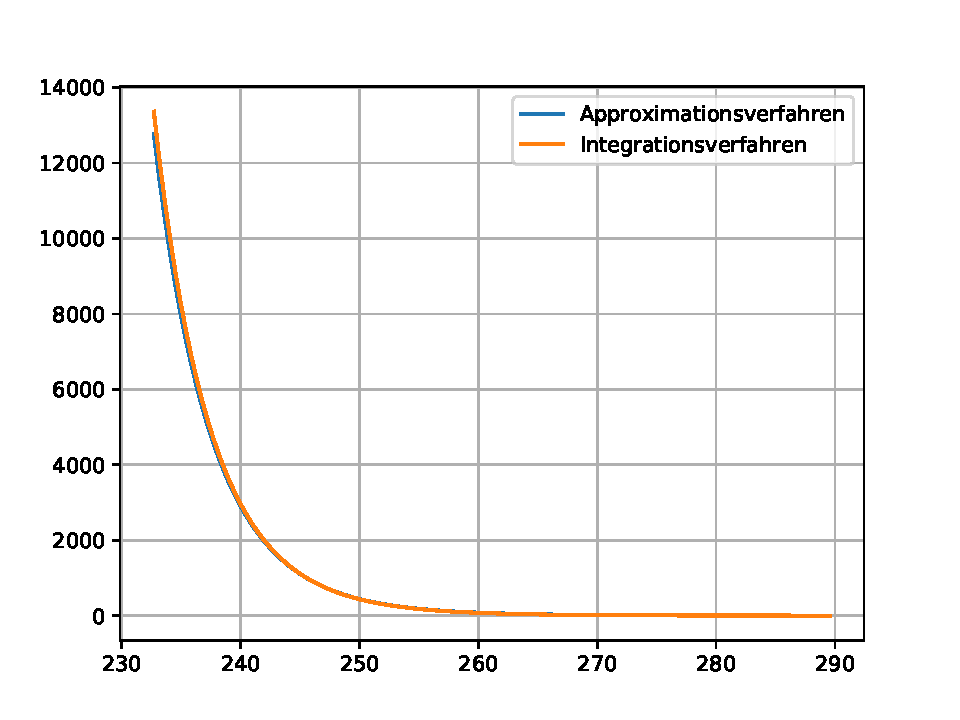
\includegraphics[width = 0.8\textwidth , keepaspectratio]{figure/tau_verlauf_B.pdf}
    \caption{Verlauf der Relaxationszeit für die Messreihe B.}
    \label{fig:tau_verlauf_B}
\end{figure}
\clearpage